%
% $Id: report.tex 52 2011-10-03 17:08:43Z justinkamerman $ 
%
% $LastChangedDate: 2011-10-03 14:08:43 -0300 (Mon, 03 Oct 2011) $ 
% 
% $LastChangedBy: justinkamerman $
%

\documentclass[10pt]{article}
\usepackage{graphicx}
\usepackage{algorithm}
\usepackage{algorithmic}
\usepackage{wrapfig}
\usepackage{caption3} % load caption package kernel first
\DeclareCaptionOption{parskip}[]{} % disable "parskip" caption option
\usepackage[font=small,format=plain,labelfont=bf,up,textfont=it,up]{caption}



\title{Document Indexing Using Aho-Corasick State Machines}
\author{Damien DuBois, Justin Kamerman, Ramanpreet Singh}
\date{\today}

\begin{document}
\maketitle

%----------------------------------------
% Abstract
%----------------------------------------
\begin{abstract}
The Aho-Corasick algorithm was originally proposed as a bibliographic
search mechanism, efficient enough to preclude the construction and
maintenance of a search index. As the size of document collections
have grown since the development of the algorithm, document
collections have grown to the point where cost of rescanning a corpus
for every search has become prohibitive and indexing, in some form or
another, is an essential optimization for any modern information
retrieval system. In this paper we demonstrate the use of
Aho-Corasick, not as an alternative to indexing but as a lexical
scanning tool employed in the construction of an inverted
index. Consistent with our analysis, an empirical evaluation of our
indexer implementation shows significant improvement over a na\"{\i}ve
algorithm. The modular architecture of our indexer allows the indexing
task to be parallelized over multiple physical nodes. The results of
parallelization are presented and offer interesting insights towards
further horizontal scaling.
\\\\
{\bf Keywords:} inverted index, Aho-Corasick state machine, finite
automata, pattern matching, parsing
\end{abstract}


%----------------------------------------
% Introduction
%----------------------------------------
\section{Introduction}
The basis of most document retrieval systems is the
term-document incidence matrix. This matrix is typically sparse and
more efficiently represented as an inverted-index which maps terms to
the parts of a document where they occur.

In order to construct an inverted index, documents must be scanned to
determine term frequencies. The Aho-Corasick string matching
algorithm\cite{RefWorks:103} is a simple and efficient text scanning
algorithm. The algorithm constructs a finite state machine to scan for
a given set of keywords. It is, in effect, a reduced grammar regular
expression parser of the type described in \cite{RefWorks:111}. The
algorithm is simple and efficient, construction time being
proportional to the sum of the length of the keyword set, and the
number of state transitions required to scan a document is independent
of the number of the size of the keyword set. In this paper we
demonstrate the use of Aho-Corasick, not as an alternative to indexing
but as a lexical scanning tool employed in the construction of an
inverted index. We provide analytic predictions of our implementation
against a na\"{\i}ve algorithm and finally, an empirical evaluation of
our inverted indexer implementation is conducted and the results
analyzed.


%----------------------------------------
% Design
%----------------------------------------
\section{Implementation}
\label{sec:implementation}
The Aho-Corasick indexer was implemented using Java and MySQL
relational database. Upon startup, the indexer reads a list of index
keywords and synonyms from the database and constructs an Aho-Corasick
state machine. The indexer then enters a loop in which it uses the
state machine to scan batches of documents retrieved from the
database. The document batch size is varied manually to match the
physical capabilities of the host. A possible enhancement to our
implementation could include an adaptive loading component. The output
of the state machine is used to augment a global index maintained in
the database.

Figure \ref{fig:deploymentmodel} shows how multiple indexer instances
can be deployed in parallel, using the database to synchronize their
access to the corpus and index. The individual indexers do not
interact directly with one another, making for a simple deployment and
operation model.


\begin{wrapfigure}{r}{0.70\textwidth}
  \begin{center}
        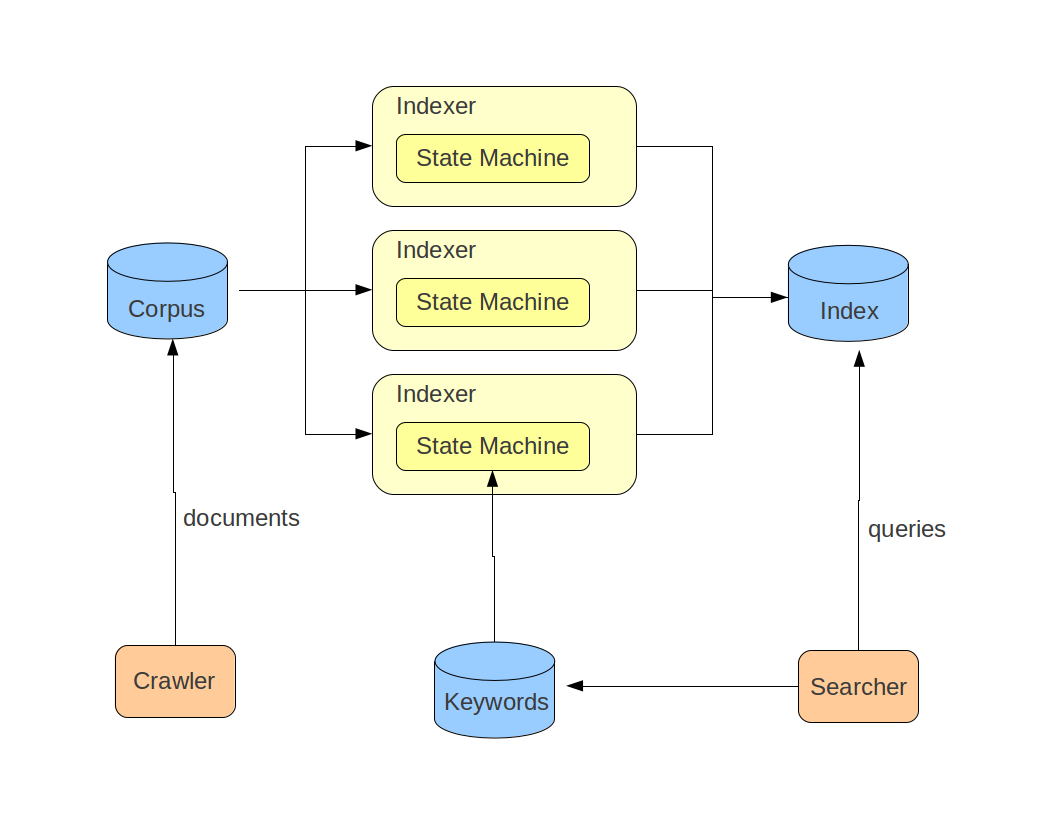
\includegraphics[width=0.70\textwidth,height=!]{deploymentmodel}
  \end{center}
  \caption{Indexer deployment model showing multiple indexer instances
  operating in parallel}
  \label{fig:deploymentmodel}
\end{wrapfigure} 

Section \label{sec:experimentresults} describes the tests conducted to
examine the effect of dictionary, document, and corpus size on the
performance of a single Aho-Corasick indexer and in \label{sec:naive}
we compare our indexer performance to that of a na\"{\i}ve
implementation. Construction time of the state machine as a function
of dictionary size was tested in order to quantify the overhead it
imposes on the indexing task. In section \ref{parallelization} we
explore the performance characteristics of a parallel indexer
deployment.

All tests were run on a single Intel Core 2 Duo 2GHz processor, 1GB
RAM, running a 64-bit Linux 2.6.35 SMP kernel. The Java Virtual
Machine used was version 1.6.0-24. 


%----------------------------------------
% Experiment Results
%----------------------------------------
\section{Experiment Results}
\label{sec:experimentresults}

%----------------------------------------
% Number of Keywords
%----------------------------------------
\subsection{Number of Keywords}
To study the impact of dictionary size on performance keywords, a
10,000 keyword dictionary of the most popular English words
\cite{wordlist} and a corpus of 50,000 blog posts of varying 
size were used. First, the time taken to construct the Aho-Corasick state
machine was measured for different numbers of dictionary keywords. The
results of this test, shown in figure
\ref{fig:numkeywordstimecomplexbuildsm}, indicate construction time to be
linear with respect to the number of keywords. This is consistent with
\cite{RefWorks:103} which formally proves that the state machine
construction algorithm is linearly proportional to the sum of the
lengths of the keywords used to construct the state machine.


\begin{figure}[ht]
  \begin{minipage}[b]{0.5\linewidth}
    \centering
    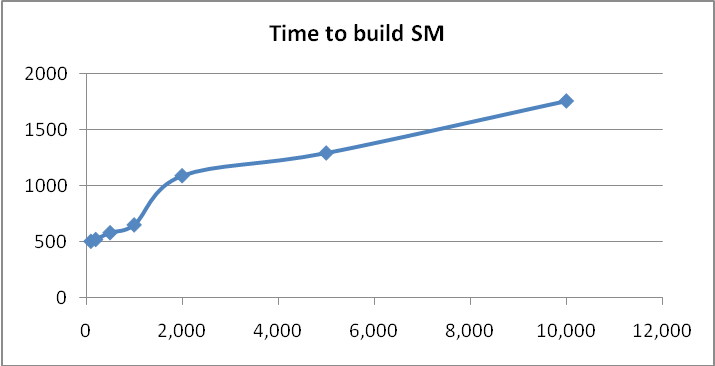
\includegraphics[width=\textwidth]{numkeywordstimecomplexbuildsm}
    \caption{Time to build Aho-Corasick state machine as a function of
      the number of keywords. Time taken is shown in milliseconds on the
      y-axis and the number of keywords on the x-axis}
    \label{fig:numkeywordstimecomplexbuildsm}
  \end{minipage}
  \hspace{0.5cm}
  \begin{minipage}[b]{0.5\linewidth}
    \centering
    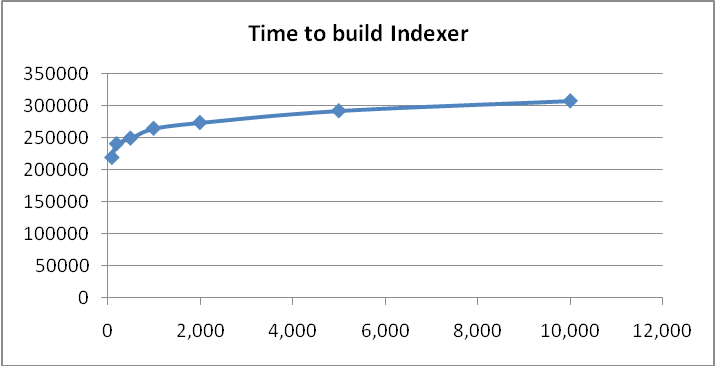
\includegraphics[width=\textwidth]{numkeywordstimecomplexbuildindex}
    \caption{Time to build the inverted index as a function of the
      number of keywords. Time taken is shown in milliseconds on the
      y-axis and the number of keywords on the x-axis}
    \label{fig:numkeywordstimecomplexbuildindex}
  \end{minipage}
\end{figure}


Second, the time taken for a state machines to build an inverted index
of our corpus was measured. The test was repeated using state machines
constructed with a varying number of keywords and the results plotted
in figure \ref{fig:numkeywordstimecomplexbuildindex}. According to
\cite{RefWorks:103}, which proves that the number of state transitions
involved in processing an input string is independent of the number of
keywords used to construct the state machine, we would not expect the
time complexity to increase with the size of the keyword set. However,
as can be seen in \ref{fig:numkeywordstimecomplexbuildindex}, the time
to build the index increases logarithmically with the number of
keywords. This is likely due to the fact that as the number of
keywords increases, so does the size of the index and the amount of
database interactions required to update the index. 

It is important to note that for this experiment, the time taken to
construct the state machine is two orders of magnitude lower than the
time taken by the indexing task. This is an important result as it
validates the practical use of the Aho-Corasick algorithm to index
large corpora, the overhead of state machine construction time being
negligible relative to the indexing task. Also, the space used by the
index in the database is proportional to the number of words we are
using. 


%----------------------------------------
% Size of Corpus
%----------------------------------------
\subsection{Size of Corpus}

\begin{wrapfigure}{r}{0.70\textwidth}
  \begin{center}
        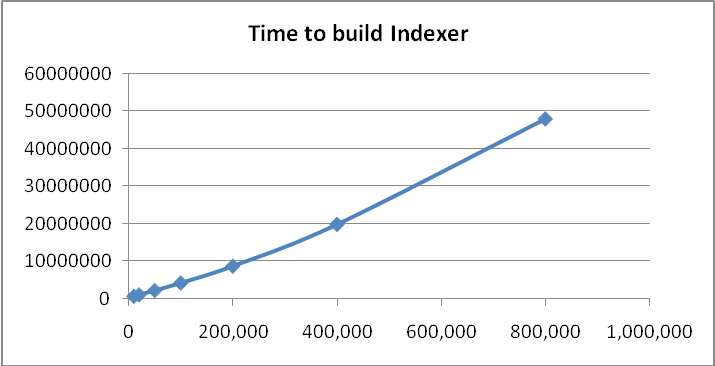
\includegraphics[width=0.70\textwidth,height=!]{corpsizetimecomplexbuildindex}
  \end{center}
    \caption{Time to build the inverted index as a function of the
      size of the corpus. Time taken is shown in milliseconds on the
      y-axis and the number of documents in the collection on the
      x-axis} 
    \label{fig:corpsizetimecomplexbuildindex}
\end{wrapfigure} 


To examine the effect of corpus size on the performance of the
indexer, a 5,000 keyword dictionary and a corpus of 800,000 blog posts
of various sizes were used. The timing results of indexing corpora of
varying sizes, shown in figure
\ref{fig:corpsizetimecomplexbuildindex}, indicate that the time to
build the index with the state machine is linear with respect to the
number of posts. 


%----------------------------------------
% Document Size
%----------------------------------------
\subsection{Document Size} 
To examine the effect of document size on indexer performance, 
a 5,000 keyword dictionary and 5,000 blog posts were used. Tests were
run in which the the size of the blog posts was varied, generating the
performance curve in figure \ref{fig:docsizetimecomplexbuildindex}.  
As expected the time to build the indexer is almost linear with
respect to the average document size.

\begin{figure}[ht]
  \begin{minipage}[b]{0.5\linewidth}
    \centering
    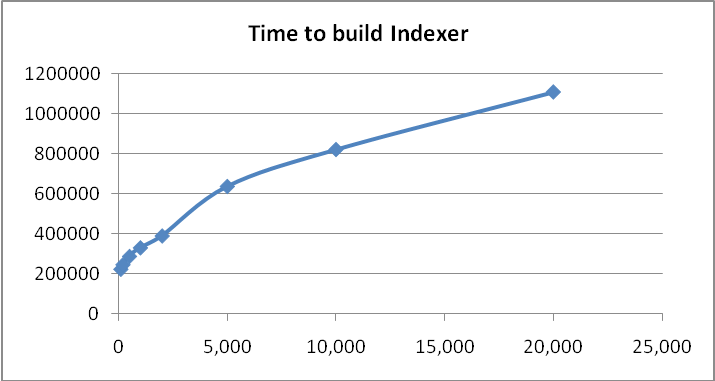
\includegraphics[width=\textwidth]{docsizetimecomplexbuildindex}
    \caption{Time to build an inverted index as a function of the
      average document size. Time taken is shown in milliseconds on the
      y-axis and the average document size in characters on the x-axis} 
    \label{fig:docsizetimecomplexbuildindex}
  \end{minipage}
  \hspace{0.5cm}
  \begin{minipage}[b]{0.5\linewidth}
    \centering
    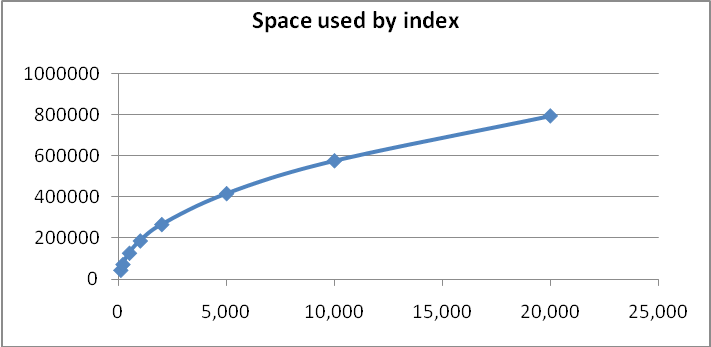
\includegraphics[width=\textwidth]{docsizespacecomplexbuildindex}
    \caption{Size of index as a function of the average document
      size. The number of database rows used to store the index is
      shown on the y-axis and the average document size in characters
      on the x-axis}  
    \label{fig:docsizespacecomplexbuildindex}
  \end{minipage}
\end{figure}

Examining the size of the index created, the larger the documents the
more records created. However, the relationship is not linear since a
single record is stored to represent one or many occurrences of a
particular keyword in a document. This relationship is shown in figure  
\ref{fig:docsizespacecomplexbuildindex}.  

%----------------------------------------
% Comparison with Naive Indexer
%----------------------------------------
\subsection{Comparison with Na\"{i}ve Indexer}
\label{sec:naive}
In order to quantify the benefits of using the Aho-Corasick algorithm
for indexing, our indexer performance was compared to that of a
na\"{i}ve implementation. The na\"{i}ve indexer builder has the same
input as our system i.e. a list of keywords and a list of documents,
and the same output i.e. an inverted index corresponding to the
keywords and documents. Algorithm \ref{alg:invertedindex} is used in
principal for both implementations. However, whereas the Aho-Corasick
implementation uses a state machine to scan, the na\"{\i}ve
indexer tokenizes the document and compares each token to the keyword
dictionary. 


\begin{algorithm}
\caption{Build inverted index}
\label{alg:invertedindex}
\begin{algorithmic}
  \FORALL{$keyword$}
  \STATE Build a vector $v$
  \FORALL {$document$}
  \IF {$keyword$ \epsilon \; $document$}
  \STATE Add the row (keyword.id, document.id) into $v$
  \ENDFOR
  \STATE Save $v$ into the database
  \ENDFOR
\end{algorithmic}
\end{algorithm}

Algorithm \ref{alg:invertedindex} has a complexity proportional to the
number of keywords $n$, the number of documents $m$, and the average
document size $\bar{c}$. For our chosen architecture, execution time
is also effected by database latency. In the case of the
na\"{\i}ve indexer, we perform one database transaction per keyword
and in the Aho-Corasick implementation, we perform a database
transaction per document. For analysis purposes, we designate the
average database latency per transaction as $\bar{t}$. 

For the na\"{i}ve indexer implementation described above, the expected
time complexity relationship is shown in equation
\ref{eqn:timecomplexworstcase}. For the Aho-Corasick indexer, the
expected theoretical complexity relationship is given by equation
\ref{eqn:timecomplexsm}.  

\begin{equation}
\label{eqn:timecomplexworstcase}
Time \propto n * ( m * \bar{c} + \bar{t} )
\end{equation}

\begin{equation}
\label{eqn:timecomplexsm}
Time \propto m * ( \bar{c}  + \bar{t} )
\end{equation}

In the context of these equations, we describe and interpret our
empirical results in the following subsections, testing for the effects
of document size $c$, number of keywords $n$, and number of documents
$m$.


%----------------------------------------
% Document Size
%----------------------------------------
\subsubsection{Document Size}
To examine the effect of document size on indexer performance, the
number of keywords was fixed at 1,000, the number of documents at
5,000, and tests run against corpora composed of varying average
length. From equations \ref{eqn:timecomplexworstcase} and
\ref{eqn:timecomplexsm}, we would expect both implementations to
behave linearly with respect to average document size and to differ by
a constant scaling factor $n$, the size of the keyword dictionary. The
experiment results are shown in figure \ref{fig:naivedocumentsize} and
support this analysis. Also, we observe that for smaller
documents, the na\"{\i}ve method performs better. This is attributable
to the fact that for smaller documents, the database advantage of the
na\"{\i}ve implementation is enough to overcome the keyword dictionary
size scaling factor. To see this effect more clearly, experiment
results are plotted on a logarithmic scale in figure
\ref{fig:naivedocumentsizelog}.


\begin{figure}[ht]
  \begin{minipage}[b]{0.5\linewidth}
    \centering
    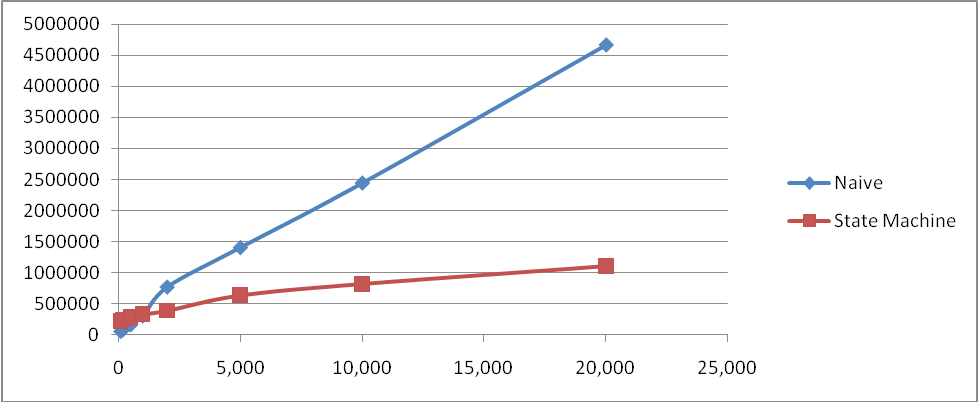
\includegraphics[width=\textwidth]{naivedocumentsize}
    \caption{Time to build an inverted index as a function of the
      average document size. Time taken is shown in milliseconds on the
      y-axis and the average document size in characters on the x-axis}
    \label{fig:naivedocumentsize}
  \end{minipage}
  \hspace{0.5cm}
  \begin{minipage}[b]{0.5\linewidth}
    \centering
    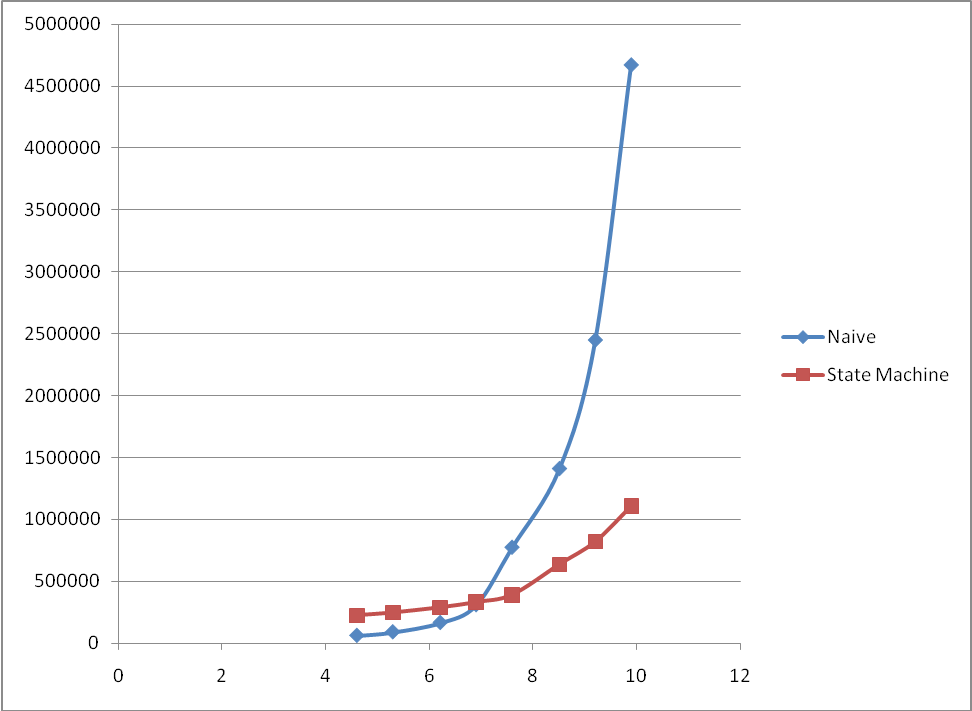
\includegraphics[width=\textwidth]{naivedocumentsizelog}
    \caption{Time to build an inverted index as a function of the
      average document size. Time taken is shown in milliseconds on the
      y-axis and the average document size in characters on the
      logarithmic x-axis}
    \label{fig:naivedocumentsizelog}
  \end{minipage}
\end{figure}


%----------------------------------------
% Keywords
%----------------------------------------
\subsubsection{Number of Keywords}
To examine the effect of keyword dictionary size on indexer
performance, the number of documents was fixed at 5,000, and tests run
using varying numbers of keywords. From equation
\ref{eqn:timecomplexworstcase}, we would expect the na\"{\i}ve
implementation to have a linear dependency on the number of keywords
and this is supported by the test results. From equation
\ref{eqn:timecomplexsm} we would not expect the Aho-Corasick
implementation to depend on the number of keyword however, the test
results seem to indicate a linear dependency. This can be attributed
to the fact that the larger the keyword dictionary, the more likely we
are to find matches in a document and incur the expensive database
latency cost.

The experiment results are shown in figure \ref{fig:naivenumkeywords}
and on a logarithmic scale in figure \ref{fig:naivenumkeywordslog}.


\begin{figure}[ht]
  \begin{minipage}[b]{0.5\linewidth}
    \centering
    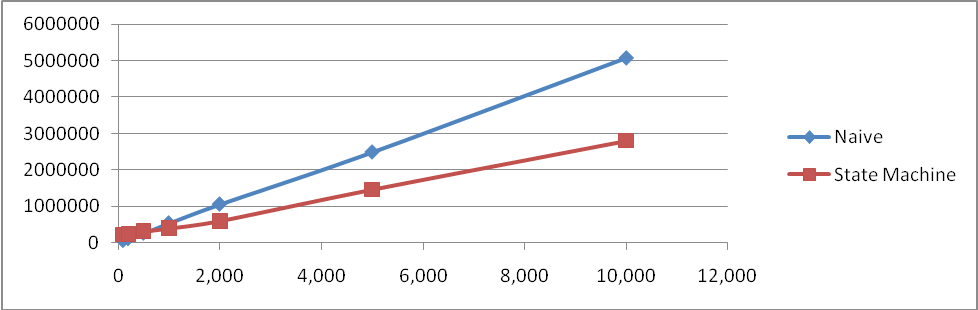
\includegraphics[width=\textwidth]{naivenumkeywords}
    \caption{Time to build an inverted index as a function of the
      number of keywords. Time taken is shown in milliseconds on the
      y-axis and the number of keywords on the x-axis}
    \label{fig:naivenumkeywords}
  \end{minipage}
  \hspace{0.5cm}
  \begin{minipage}[b]{0.5\linewidth}
    \centering
    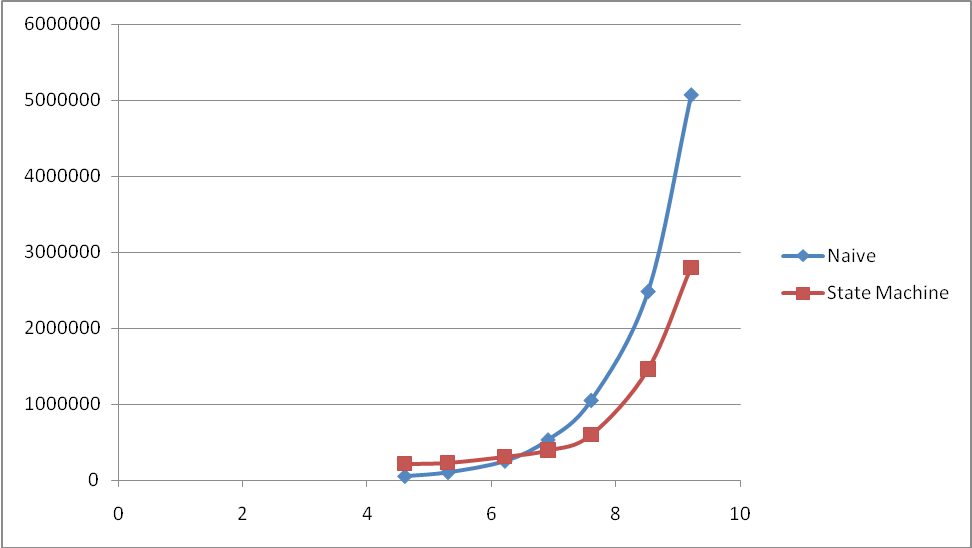
\includegraphics[width=\textwidth]{naivenumkeywordslog}
    \caption{Time to build an inverted index as a function of the
      number of keywords. Time taken is shown in milliseconds on the
      y-axis and the number of keywords on the logarithmic x-axis}
    \label{fig:naivenumkeywordslog}
  \end{minipage}
\end{figure}


%----------------------------------------
% Corpus Size
%----------------------------------------
\subsubsection{Number of Documents}
From equations \ref{eqn:timecomplexworstcase} and
\ref{eqn:timecomplexsm}, the time complexity is linearly related to
the number of documents being indexed. The experiment results, in this
respect, are shown in figure \ref{fig:naivesizecorpus} and on a
logarithmic scale in figure \ref{fig:naivesizecorpuslog}.

\begin{figure}[ht]
  \begin{minipage}[b]{0.5\linewidth}
    \centering
    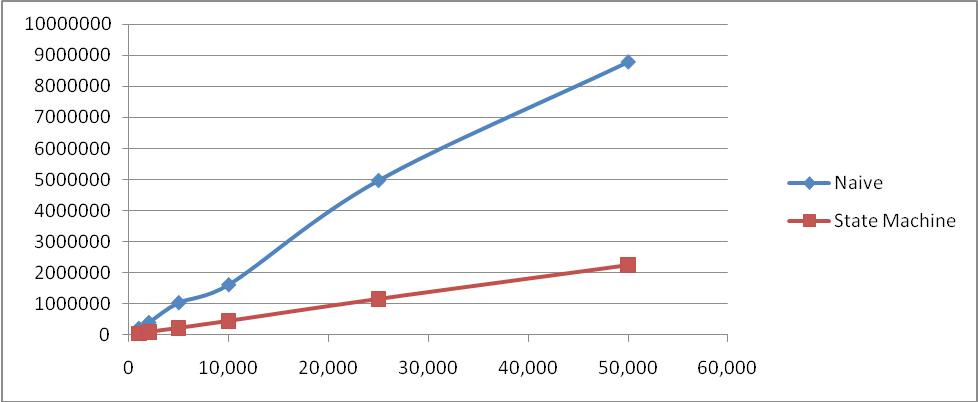
\includegraphics[width=\textwidth]{naivesizecorpus}
    \caption{Time to build an inverted index as a function of the
      number of documents being indexed. Time taken is shown in
      milliseconds on the y-axis and the number of documents on the
      x-axis} 
    \label{fig:naivesizecorpus}
  \end{minipage}
  \hspace{0.5cm}
  \begin{minipage}[b]{0.5\linewidth}
    \centering
    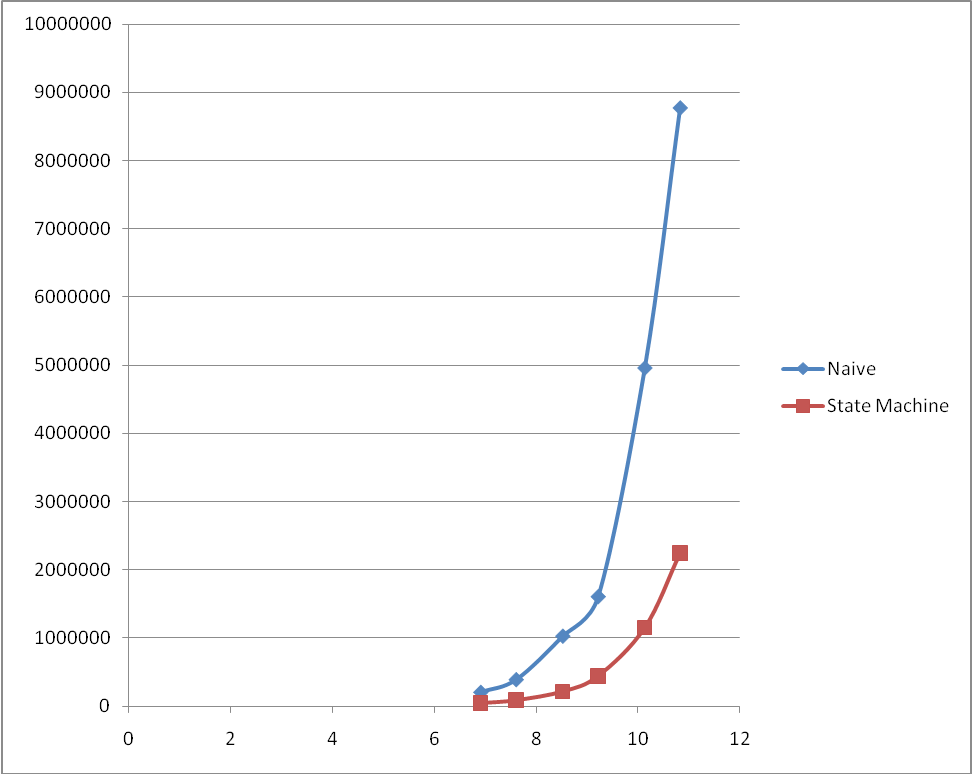
\includegraphics[width=\textwidth]{naivesizecorpuslog}
    \caption{Time to build an inverted index as a function of the
    number of documents being indexed. Time taken is shown in
      milliseconds on the y-axis and the number of documents on the
      logarithmic x-axis} 
  \label{fig:naivesizecorpuslog}
  \end{minipage}
\end{figure}



%----------------------------------------
% Parallelization
%----------------------------------------
\subsection{Parallelization}
\label{parallelization}
Given the modular architecture of our indexer, it is possible to
deploy multiple instances of the program to work concurrently on the same
indexing task. The instances interact via the database which
synchronizes their operations on the corpus and the index itself. To
investigate the effect of parallelization on the indexer operation, the
indexer was deployed using a single database server storing documents,
keywords, and the resulting index. Four indexer nodes were used, each
running a single instance of the indexer program. 

In this experiment a corpus of 100,000 documents and 1000 keywords were
used, each document 5000 words in length. Tests were run using various
node combinations and the time taken to index the corpus was measured and
normalized to a throughput metric (documents/second) for convenient
comparison and to account for differences in the physical capabilities
and configuration of the worker nodes. A series of tests were
performed using a corpus of 800,000 documents to investigate the
effect of corpus size on performance. The results of this experiment
are shown in figure \ref{fig:parallelization}.


\begin{wrapfigure}{r}{0.70\textwidth}
  \begin{center}
        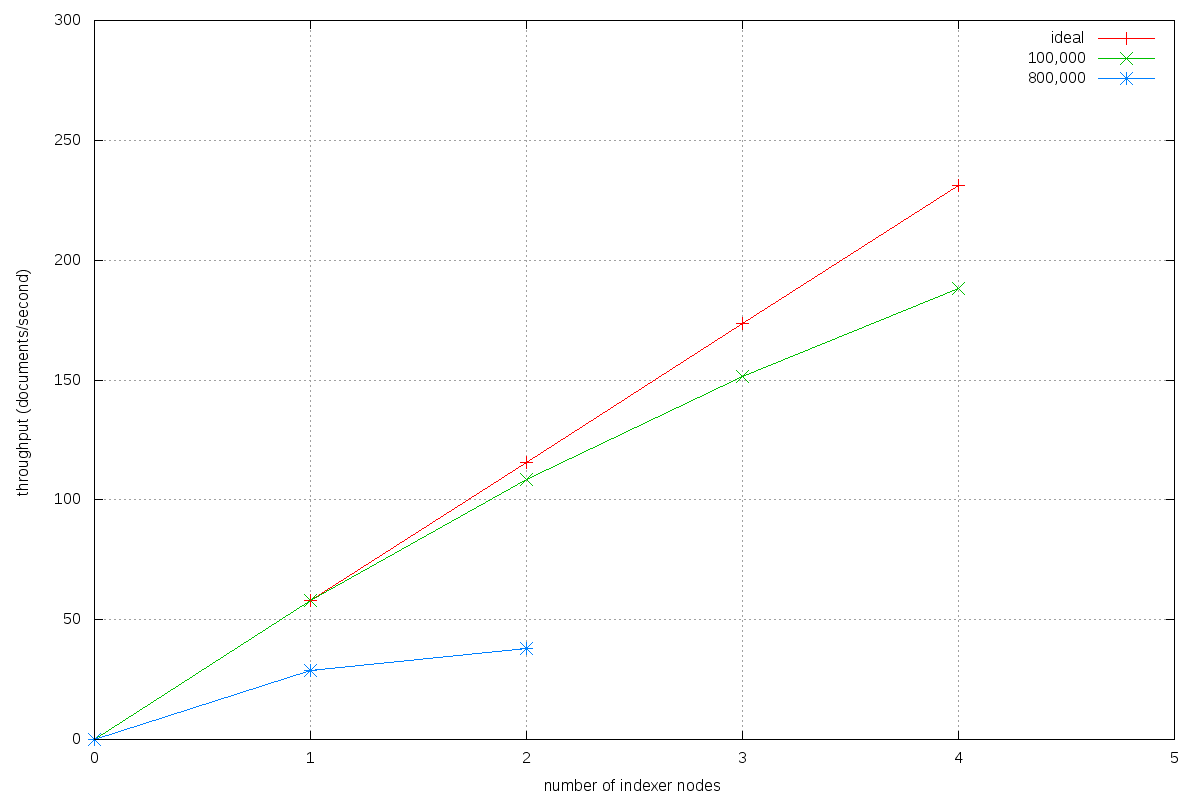
\includegraphics[width=0.60\textwidth,height=!]{parallelization}
  \end{center}
  \caption{Performance characteristics of parallel indexer
    deployment. The \textit{ideal} curve shows the theoretical
    performance curve based on linear combination of average
    individual node performance over the corpus} 
  \label{fig:parallelization}
\end{wrapfigure} 


For the 100,000 document corpus, increasing the number of nodes
increases throughput but with diminishing returns. As the database
connection pool is saturated, this becomes the limiting factor of the
architecture. If the number of nodes were increased further, one would
expect the curve to plateau at some point. After this point, adding
additional nodes would offer no improvement and may even decrease
performance as the worker processes spend an increasing amount of time
context switching and contending for locks. These factors could be
mitigated up to a point by increasing batch sizes and tuning the
database. However, the characteristics of the curve are ultimately
unavoidable in the current architecture. 

For the 800,000 document corpus, the performance curve shows an even
more severe degradation than the smaller corpus. Since we normalize
the performance metrics for the size of the document collection, one
would expect this curve to be more similar to that of the 100,000
document collection. A possible explanation for the deviation is that
for the larger collection, more documents were present in the
database and the resulting index larger. This results in longer table
scan times to retrieve and update records. This effect could be
alleviated through the use of indices and other database optimization
techniques, however, as for the smaller document
collection, this degradation is ultimately unavoidable.


%----------------------------------------
% Conclusions
%----------------------------------------
\section{Conclusions}
\label{sec:conclusions}
The experimental results tend to prove what we could expect from
theory. Our system is faster than the na\"{i}ve indexer with respect
to the number of keywords being indexed, size of the document
collection, and average document size. In particular, our indexer
implementation performs relatively well with respect to the number of
documents being indexed. Moreover, as soon as we are dealing with a number of
keywords that can be representative of real-world needs, the state
machine implementation proves also to be significantly faster than the
naive indexer. 

One of the primary goals of this research project was to leverage the
effect of parallelization in reducing the time to index a document
collection. We successfully demonstrated that performance gains could
be achieved for the indexing task through parallelization as well as
the fact that our architecture offers diminishing returns as the
number of nodes is increased and as the corpus becomes larger.

 Other avenues of interest include, but are not limited
to:

\begin{itemize}
  \item Compare the Aho-Corasick state machine indexer implementation
    to less na\"{i}ve indexer implementations.
    
    \item Use compression techniques to our algorithm in order to
      reduce the index size in the database.

      \item Conduct further parallelization experiments to determine
        the performance characteristics of our indexer over a wider
        range of operating conditions.

    \item Study the time performance improvements possible deploying
      the Aho-Corasick state machine indexer within a commercial
      \textit{MapReduce} framework such as \textit{Hadoop}.
\end{itemize}



%----------------------------------------
% Bibliography
%----------------------------------------
% changes default name Bibliography to References
\renewcommand\bibname{References}
\bibliography{bibliography}
\bibliographystyle{IEEEannot}

\end{document}
